% !TEX root = ../../thesis.tex


\newpage
\phantom{}
\thispagestyle{empty}
\section{A one dimensional model for Wave Turbulence}
    The Majda-McLaughlin-Tabak (MMT) family of models was introduced in \cite{Majda1997} to test the prediction of weak turbulence theory. The idea is to have a 1D system manifesting
    the main phenomenology of nonlinear physics, while at the same time being relatively easy to numerically simulate on a fine grid. Its study was then continued in
    \cite{Cai2001} and \cite{Zakharov2001}, and resulted in a better understanding of how coherent phenomena (like solitons or quasisolitons) influence the applicability 
    of wave turbulence theory. This two parameters family of models has since been a traditional benchmark on which to test new techniques and ideas in the world of turbulence. \\
    In this chapter, we briefly introduce the MMT family of differential equations and discuss its salient features and associated WKE, mainly inspired by the account in 
    \cite{ZAKHAROV2004}. We then 
    move to the analysis of its higher order kinetic equation, proving that energy and wave action are still conserved quantities. Unexpectedly,  we find 
    ulterior divergences, neither UV nor IR, due to nonlocal interactions. We prove that for all nontrivial members of the MMT family of
    models these divergences exist, and must be accounted for. Our original idea was to perform numerical simulations of the higher order WKE, to check the form of eventual out of equilibrium stationary states. This newly found diverging integrals didn't allow us to do so. Nonetheless, we introduce the basic workings of WavKinS,
    a newly developed solver for WKEs introduced in \cite{Giorgio1} and \cite{Giorgio2} by Krstulovic. We end the chapter by discussing some simulations of the leading order WKE. 
    \newpage  
    \vphantom{a}
    \subsection{The MMT model}

    The model consists, in physical space, in the two parameters family of differential equations
    \begin{equation}
        i\pt \Psi = \left|\px\right|^\alpha \Psi + \lambda \left|\px\right|^{\frac{\beta}{4}}
        \left( \left|\left|\px\right|^{\frac{\beta}{4}}\Psi\right|\left|\px\right|^{\frac{\beta}{4}}\Psi \right),
        \label{MMTPOS}
    \end{equation}
    where $\Psi = \Psi(x,t)$ is a complex function, $\lambda = \pm 1$ and $\alpha, \beta \in \mathbb{R}$. Positive $\lambda$ 
    corresponds to the defocusing case whereas negative $\lambda$ to the focusing one.\\
    We interpret the fractional derivatives in \eqref{MMTPOS} through their action in Fourier space, namely 
    \begin{equation}
        \left|\px\right|^\alpha \Psi = \frac{1}{2\pi} \int dk |k|^{\alpha} a_k e^{-ikx},
    \end{equation} 
    where $a_k = \anorm(k,t)$ is the Fourier transform of $\Psi$. A rigorous definition can be found in the appendix of \cite{ZAKHAROV2004}\\
    Time translational symmetry implies that the energy
    \begin{equation}
        \Ewav = \int dx \left( \left|\left|\px\right|^\frac{\alpha}{2}\Psi\right|^2 + \frac{1}{2}\lambda\left|\left|\px\right|^\frac{\beta}{4}\Psi\right|^4 \right)
    \end{equation}
    is conserved. Phase and translational symmetries corresponds instead to the conservation of wave action/number and momentum, with formulas
    \begin{equation}
        \Nwav = \int dx \left| \Psi \right|^2 \hspace{1cm} \textrm{M} = \frac{i}{2}\int dx \left( \Psi \px \Psi^* - \Psi^* \px \Psi \right).
    \end{equation}
    Transforming \eqref{MMTPOS} to Fourier space we find
    \begin{equation}
        i\pt \ak = \omga_k \ak  + \int dk_1dk_2dk_3 \Tint_{k123}\aone \atwo \athreestar \delta^{k1}_{23}.
    \end{equation}
    There, to have uniform notation with the previous chapters, we defined\footnote{As this model is one dimensional $k$ is the only component of the wave vector and $|k|$ its modulus.} $\omga_k = |k|^\alpha$ and $\Tint_{k123} = \lambda|kk_1k_2k_3|^\frac{\beta}{4}$. It is easy to see that
    $\Tint$ satisfies the symmetries generally required in chapter 1, allowing for the Hamiltonian treatment of the system. \\
    This system possess by construction only a four wave interaction. In one dimension the resonance condition is
    \begin{equation}
        \begin{aligned}
            k + k_1 &= k_2 + k_3 \\
            |k|^\alpha + |k_1|^\alpha &= |k_2|^\alpha + |k_3|^\alpha.
        \end{aligned}
    \end{equation}
    In \cite{Majda1997} it was proved that the only way nontrivial solution exists\footnote{
        A nontrivial solution is a solution which does not make the collision integral null, and thus result in an exchange of energy among modes. 
        For example $k=k_2$ and $k_1=k_3$ is always a solution, but the term 
        $\left(\frac{1}{n_k} +\frac{1}{n_1} -\frac{1}{n_2}-\frac{1}{n_3} \right)$ kills the collision integral in that point of the resonance manifold.
    } is if $\alpha < 1$. We shall then adopt $\alpha = \frac{1}{2}$ to mimic the dispersion relation of surface gravity waves, in which case $\omga = |gk|^\frac{1}{2}$ 
    with $g$ being the acceleration of gravity.\\
    By direct substitution of MMT's dispersion relation and interaction term into $\eqref{kinetic}$, the WKE to the leading order is 
    \begin{multline}
        \pt n_k = 4 \pi\int dk_1 dk_2 dk_3 
        |kk_1k_2k_3|^\frac{\beta}{2}
        \\ \times n_kn_1n_2n_3
    \left(\frac{1}{n_k} + \frac{1}{n_1} - \frac{1}{n_2}- \frac{1}{n_3}  \right)
    \delta(\delomega^{k1}_{23})\delta^{k1}_{23}.
    \end{multline}
    Given that the model is one dimensional we will refer with $k$ to the value of the only component of the wave vector, when talking about its modulus we shall use $|k|$ instead. The isotropy assumptions would correspond in one dimension
    to the reflection symmetry $k \rightarrow -k$.\\ 
    From the discussion in chapter 1 we know that the two possible out of equilibrium solutions for this equation are 
    \begin{equation}
        \begin{aligned}
        &n_k^P \propto |k|^{\frac{2}{3}\beta + 1}, \\
        &n_k^Q \propto |k|^{\frac{2}{3}\beta + \frac{5}{6}}.
        \end{aligned}
        \label{MMTKZ}
    \end{equation}
    Since the interaction term appears squared in the WKE, weak turbulence theory provides the same prediction in both the focusing and defocusing cases. 
    However, \eqref{MMTPOS} presents different behaviors depending on the sign of the interaction. 
    In the focusing case stable solitonic solutions are possible, as well as wave collapses
    (\cite{Zakharov2001}). It was seen in numerical simulations of the primitive equation that, under incoherent forcing, the wave density spectrum stabilizes in a state
    with opposite wave action flux respect to the WT prediction. The energy flux sign corresponds to predictions, but only in the high $k$ limit the slope can be 
    described through a KZ state.\\
    In the defocusing case the spectrum qualitatively corresponds to the expected one, but with a steeper slope in the inertial range. This discrepancy could be justified 
    by the presence of quasi solitons, approximate solutions of \eqref{MMTPOS} dissipating in finite time. The study of their impact on stationary states is called 
    quasisolitonic turbulence. \\
    These considerations show that the range of applicability of WT is quite narrow, and very much influenced by the coherent structures characteristic of the system under analysis. 
    Our goal in this thesis is not to discuss the validity of WT, but instead check the consistency and study consequences of the presence of higher order terms into the 
    WKE of a simple system. We shall direct the reader looking for a proper discussion of 
    coherent phenomena in the MMT model to \cite{ZAKHAROV2004}. \\
    \subsection{The higher order kinetic equation}

    By directly substituting our chosen dispersion relation and interaction term into \eqref{NLOkinetic}, the next to leading order kinetic equation for the MMT 
    model is 
    \begin{multline}
        \frac{\partial}{\partial t}n_k(t) = 4\pi \int dk_1dk_2dk_3[1 + \sigma(k,k_1,k_2,k_3)]\\
        \times |kk_1k_2k_3|^{\beta/2} n_kn_1n_2n_3 \left(\frac{1}{n_k} +\frac{1}{n_1}-
        \frac{1}{n_2}-\frac{1}{n_3}\right)\delta_{23}^{k1}\delta(\delomega^{k1}_{23}), 
        \label{wke_nlo}
    \end{multline}
    where 
    \begin{multline}
        \sigma(k,k_1,k_2,k_3) =  4 \int dk_4dk_5n_4n_5|k_4k_5|^{\beta/2} \\
        \times \left[\left( \frac{1}{n_4}+\frac{1}{n_5} \right) 
        \frac{\delta_{23}^{45}}{\sqrt{k_2}+\sqrt{k_3}-\sqrt{k_4}-\sqrt{k_5}} \right.
        \\ + 4\left( \frac{1}{n_4}-\frac{1}{n_5} \right) 
        \left.\frac{\delta_{14}^{35}}{\sqrt{k_3}+\sqrt{k_5}-\sqrt{k_1}-\sqrt{k_4}}\right].
        \label{sigma}
    \end{multline}
    We rewrote the equation in this fashion to highlight the contributions of higher perturbative orders as modifications to the effective interaction term in the WKE.
    If we imagine the leading order WKE as accounting for all possible scatterings among waves, the $\sigma$ term here introduced accounts for secondary scatterings 
    mediated by some virtual waves $k_4$ and $k_5$. The full effect is to either suppress or enhance the interaction, resulting in a new coupling 
    \begin{equation*}
    |kk_1k_2k_3|^{\beta/2} \longrightarrow [1 + \sigma(k,k_1,k_2,k_3)]|kk_1k_2k_3|^{\beta/2} . 
    \end{equation*}
    The leading order WKE conserves energy and wave action as consequences of the symmetries of $\Tint_{k123}$. To show that even the corrected equation 
    conserves the same quantities, as it is expected, we shall just check that the same symmetries hold for $\sigma$.\\
    The symmetry under the exchange $k_2 \leftrightarrow k_3$ is built-in but not explicit, as already commented in the previous chapter. The contribution of the 
    first diagram in figure \ref{fig:quarticoneloop} is obviously symmetric, and the other two contribution are mapped into each other by the exchange. It was used to make
    \eqref{NLOkinetic} more compact. \\
    Recovering it and manipulating the dummy variables, 
    $\sigma$ becomes
    \begin{multline}
      \sigma(k,k_1,k_2,k_3) =  4 \int dk_4dk_5n_4n_5|k_4k_5|^{\beta/2} \\
       \times \left[\left( \frac{1}{n_4}+\frac{1}{n_5} \right) 
      \frac{\delta_{23}^{45}}{\sqrt{k_2}+\sqrt{k_3}-\sqrt{k_4}-\sqrt{k_5}} \right.
      + \left( \frac{1}{n_4}-\frac{1}{n_5} \right) \\ 
      \times\left(\frac{\delta_{14}^{35}}{\sqrt{k_3}+\sqrt{k_5}-\sqrt{k_1}-\sqrt{k_4}} - \frac{\delta_{15}^{34}}{\sqrt{k_3} 
       +\sqrt{k_4}-\sqrt{k_1}-\sqrt{k_5}}  \right. \\
      \left. \left. +\frac{\delta_{14}^{25}}{\sqrt{k_2}+\sqrt{k_5}-\sqrt{k_1}-\sqrt{k_4}} -\frac{\delta_{15}^{24}}{\sqrt{k_2}
      +\sqrt{k_4}-\sqrt{k_1}-\sqrt{k_5}}\right)\right].
      \label{eqsym}
    \end{multline}
    Under the exchange $(k \text{,} k_1) \leftrightarrow (k_2 \text{,} k_3)$  we obtain
    \begin{multline}
      \sigma(k,k_1,k_2,k_3) =  4 \int dk_4dk_5n_4n_5|k_4k_5|^{\beta/2} \\
       \times \left[\left( \frac{1}{n_4}+\frac{1}{n_5} \right) 
      \frac{\delta_{1k}^{45}}{\sqrt{k}+\sqrt{k_1}-\sqrt{k_4}-\sqrt{k_5}} \right. 
      + 4\left( \frac{1}{n_4}-\frac{1}{n_5} \right) \\
      \times \left(\frac{\delta_{34}^{15}}{\sqrt{k_1}+\sqrt{k_5}-\sqrt{k_3}-\sqrt{k_4}} - \frac{\delta_{35}^{14}}{\sqrt{k_1} +\sqrt{k_4}-\sqrt{k_3}-\sqrt{k_5}}  \right. \\
      \left. \left. +\frac{\delta_{34}^{k5}}{\sqrt{k}+\sqrt{k_5}-\sqrt{k_3}-\sqrt{k_4}} -\frac{\delta_{35}^{k4}}{\sqrt{k}+\sqrt{k_4}-\sqrt{k_3}-\sqrt{k_5}}\right)\right].
    \end{multline}
    Imposing $\omega + \omega_1 = \omega_2 +\omega_3$ and $k + k_1 = k_2 + k_3$ results in
    \begin{multline}
      \sigma(k,k_1,k_2,k_3) =  44 \int dk_4dk_5n_4n_5|k_4k_5|^{\beta/2} \\
       \times \left[\left( \frac{1}{n_4}+\frac{1}{n_5} \right) 
      \frac{\delta_{1k}^{45}}{\sqrt{k_2}+\sqrt{k_3}-\sqrt{k_4}-\sqrt{k_5}} \right. 
      + \left( \frac{1}{n_4}-\frac{1}{n_5} \right) \\
      \times \left(\frac{\delta_{34}^{15}}{\sqrt{k_1}+\sqrt{k_5}-\sqrt{k_3}-\sqrt{k_4}} - \frac{\delta_{35}^{14}}{\sqrt{k_1} +\sqrt{k_4}-\sqrt{k_3}-\sqrt{k_5}}  \right. \\
      \left. \left. +\frac{\delta_{25}^{14}}{\sqrt{k_2}+\sqrt{k_5}-\sqrt{k_1}-\sqrt{k_4}} -\frac{\delta_{24}^{15}}{\sqrt{k_2}+\sqrt{k_4}-\sqrt{k_1}-\sqrt{k_5}}\right)\right],
    \end{multline}
    showing that $\sigma(k,k_1,k_2,k_3) = \sigma(k_2,k_3,k,k_1) = \sigma(k,k_1,k_3,k_2)$ and thus that $E$ and $N$ are conserved\footnote{
    We do not need to prove directly symmetry under $k \leftrightarrow k_1$, as it is implied by the other two combined.}.\\ 
    There are two integrations in \eqref{wke_nlo}, an external one (three integration measures with two deltas) and an internal one (two measures with one delta). 
    To assess the validity of a possible stationary solution one should check the convergence of both integrals in all possible regimes of their arguments.\\ One could also
    slightly deform one of solutions \eqref{MMTKZ}, and assess qualitatively the contribution of $\sigma$ to the KZ spectrum. This line of thought 
    was explored for the NLS equation in \cite{Rosenhaus:2025mgj}. We shall not discuss this points here. Even before thinking about specific solutions 
    the integrals have to converge for a generic $n_k$, allowing for non-pathological time evolution.\\
    In this thesis we shall not concern ourselves with IR and UV divergences,
    as those are easily healed through cutoffs. Those cutoffs may derive from the underlying physics of the system under consideration, for example 
    finite size imposes a natural UV cutoff and granularity of the medium imposes an IR one. They could be even imposed by the interactions of the system with 
    the environment, for example a dissipative interaction in the low $k$ region denies the transfer of energy or wave action across its domain. \\
    We shall instead focus our attention on the denominators of $\sigma$. Their integration should be intended in the principal value sense, but this only allows to 
    assign a value to usually indeterminate integrals. We have to explicitly check that this value is finite. We shall turn to this problem for the remaining part 
    of this section.\\

    Let us look at the first term in \eqref{sigma}
    \begin{equation}
        \frac{\delta_{23}^{45}}{\sqrt{k_2}+\sqrt{k_3}-\sqrt{k_4}-\sqrt{k_5}},
    \end{equation} 
    as we already said we can interpret the $\sigma$ term as the exchange of virtual waves among different modes.
    $k$ and $k_1$ produce two virtual waves ($k_4$ and $k_5$) that rescatter into $k_2$ and $k_3$.
    Being virtual they do not need to be resonant, but the closer to resonant they are, the bigger their contribution to the process, as the denominator suggests.   
    We recast it by using the delta function in the numerator, removing in the process the $k_5$ integration, and rename $k_4=q$. Remember that $\sigma$ arguments $k\dots k_3$ have to be part of the resonant manifold, hereby called external, implying  that the first denominator
    \begin{equation}
        \begin{aligned}
      D_1 &= \sqrt{k_2} + \sqrt{k_3} -\sqrt{q} - \sqrt{k_2 + k_3 - q}\\
       &= \sqrt{k} + \sqrt{k_1} -\sqrt{q} - \sqrt{k + k_1 - q}.
        \end{aligned}
    \end{equation}
    It is easy to see that this expression has four zeroes corresponding to $q$ equal to any of the external wave vectors. \\
    As long as $k \neq k_1$ or $k_2 \neq k_3$ the zeroes are singles. For example let's look at $q = k$. We rename $p = q-k$ and expand around $p=0$:
    \begin{align*}
      \sqrt{|k|} + \sqrt{|k_1|} -\sqrt{|p+k|} - \sqrt{|k_1 - p|} \underset{p \rightarrow 0}{\approx} \frac{1}{2} p \left(\frac{\text{sign}(k)}{\sqrt{|k|}} - \frac{\text{sign}(k_1)}{\sqrt{k_1}}\right).
    \end{align*}
    In this case $\int dp\frac{1}{D}$ would behave close to $p=0$ as $\int_{-\epsilon}^{+\epsilon}\frac{dp}{p}$, whose Cauchy principal value is 0. \\
    If $k_1 = k$ we have to move to second order in the expansion, finding 
    \begin{equation}
      2\sqrt{|k|} -\sqrt{|p+k|} - \sqrt{|k - p|} \underset{p \rightarrow 0}{\approx} \frac{1}{2}|k|^{-\frac{3}{2}} p^2.
    \end{equation}
    This is a problem, as the principal value of $\int_{-\epsilon}^{+\epsilon}\frac{1}{p^2}$ diverges.\\
    We must remember that the $\sigma$ term is multiplied to $\frac{1}{n_k} + \frac{1}{n_1} -\frac{1}{n_2} -\frac{1}{n_3}$ in the full kinetic equation. This means that if in the external manifold $k = k_1$ implies $k_2 = k_3$, the divergence in $\sigma$ can be healed by a zero in the kinetic equation. If instead there are nontrivial points where $k=k_1$ corresponds to $k_2 \neq k_3$, we are looking at a true divergence.\\
    We set $k_1=k$ in the equations defining the external resonant manifold, the system to solve is thus
    \begin{equation}
        \begin{aligned}
            &2k = k_2 + k_3 \\
            &2\sqrt{|k|} = \sqrt{|k_2|} + \sqrt{|k_3|}
        \end{aligned}
        \label{resmanifold}
    \end{equation}
    Assuming $k>0$ there is the trivial solution ($k_2 = k_3 = k$) and two nontrivial ones,
    $k_2 = -\frac{k}{4} \hspace{1mm} \& \hspace{1mm}k_3 = \frac{9k}{4} $ and $k_3 = -\frac{k}{4} \hspace{1mm}\& \hspace{1mm}k_2 = \frac{9k}{4} $ that can be found by direct substitution of the first equation into the second. The sign of the integrand is the same in both cases not allowing for possible cancellations.  This confirms our fears, making the $\sigma$ term divergent.\\
    One may wonder if with a different dispersion relation the situation changes. We shall approach the problem geometrically.
    With generic $\alpha$ the second equation turns into 
    \begin{equation}
      2|k|^{\alpha} = |k_2|^{\alpha} +|k_3|^{\alpha}.
      \label{frequency}
    \end{equation} 
    The first equation in \eqref{resmanifold} can be thought of as a line $k_3 = -k_2 + 2k$, with $k_2$ on the $x$ axis, $k_3$ on the $y$ one and $2k$ a constant. The second equation implicitly defines  a curve, specular under both $k_2 \rightarrow -k_2$ and $k_3 \rightarrow -k_3$. The line intersect the deformed sphere in the trivial solution of the system $k_2 = k_3 = k$, that depending on the sign of $k$ can be either in the upper right quadrant or in the lower left one. Using Dini's theorem on implicit functions, we can evaluate the first derivative of $k_3$ as a function of $k_2$. The result is 
    \begin{equation}
        \frac{d k_2}{dk_3} = -\frac{\text{sign}(k_2)|k_2|^{\alpha-1}}{\text{sign}(k_3)|k_3|^{\alpha-1}}.
        \label{firstderivative}
    \end{equation}
    Substituting the trivial solution we see that the first derivative is $-1$ in the intersection point, same as the line's slope, meaning they are tangent in that point. We can also see from \eqref{firstderivative} that in each quadrant the implicit function defined by \eqref{frequency} is monotonical. This gives us a way to check if nontrivial solutions are possible. If the curve is 
    convex in each quadrant there are no other possible intersections with the line, as moving away from the trivial one will keep increasing the distance between the curve and the line, with the curve being closer to the origin. When the curve reaches one of the other quadrants the derivative changes sign, bringing the curve even far away from the prosecution of the line in that quadrant. If instead the curve is concave the inverse is true, as the curve will grow farther from the origin than the line. This will impose two intersections in the adjacent quadrants, where the derivative changes sign.\\
    Using an extension of Dini's theorem, we can evaluate the second derivative. We do so in the upper right quadrant, as the reflection symmetry of the problem extend the result to the lower left one. We obtain 
    \begin{equation}
        \frac{d^2k_3}{dk_2^2} = \frac{(1-\alpha)k_2^{\alpha-2}k_3^{2\alpha-2} + (1-\alpha)k_3^{\alpha-2}k_2^{2\alpha-2}}{k_3^{3\alpha-3}}.
    \end{equation}   
    We see from this result that the second derivative sign does not change throughout the quadrant and is positive when $\alpha < 1 $, making the curve concave and allowing nontrivial solutions, and negative when $\alpha > 1$, forbidding solutions other than $k_3 = k_2 = k$. Since the resonant manifold is empty for $\alpha>1$, the aforementioned divergences are always present for the nontrivial set of MMT models. Our construction is presented in figure \ref{fig:nonlocal}.\\
    This line of reasoning does hold for $k_2 = k_3$ as well.\\
    \begin{figure}[ht]
        \centering
        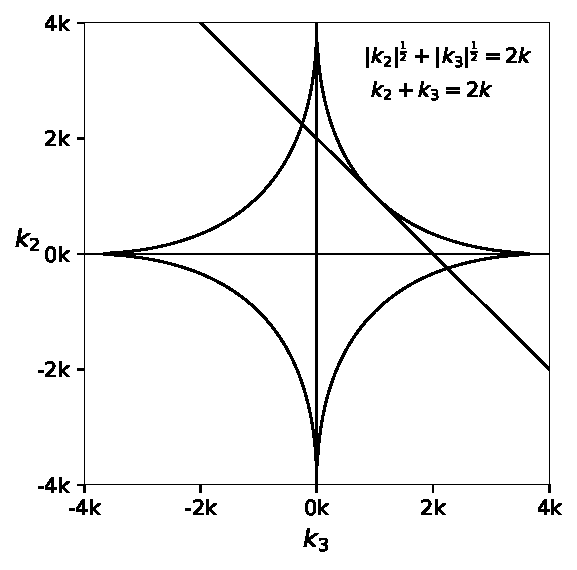
\includegraphics[width=0.4\textwidth]{images/nonlocal_resonances_convex.pdf}
        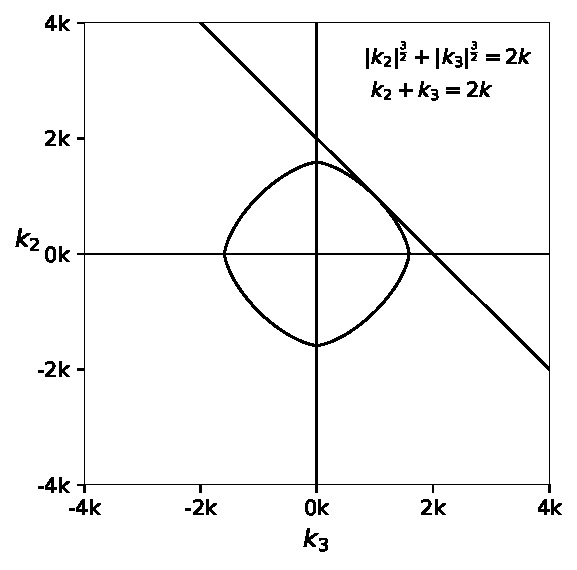
\includegraphics[width=0.4\textwidth]{images/nonlocal_resonances_concave.pdf}
        \caption{Examples of resonant manifolds when $k_1 = k$, in the cases $\alpha = \frac{1}{2}$ and $\alpha = \frac{3}{2}$. In the first case there are two nontrivial interactions.}
        \label{fig:nonlocal}
    \end{figure}
    Moving to the second denominator, and again exploiting the delta function and renaming $k_4 = q$, we study
    \begin{equation}
        \begin{aligned}
      D_2 &= \sqrt{k} - \sqrt{k_2} - \sqrt{|q|} + \sqrt{|k_2-k + q|} \\
      &= \sqrt{k_3} - \sqrt{k_1} - \sqrt{|q|} + \sqrt{|k_1-k_3 + q|}
        \end{aligned}
    \end{equation}
    we see that it is null for $q = k_3$ and $q = k$. Recovering the symmetry part as in \eqref{eqsym} we would find a similar expression with divergences in $q = k_1$ and $q = k_2$. \\
    Again when no external wave vectors collide the divergent part goes as $\int_{-\epsilon}^{+\epsilon}\frac{1}{p}$ and its principal value is null. When $k_1 = k_3$ or $k = k_3$ there is yet another singularity whose principal value diverges. This one is however balanced by the term $\frac{1}{n_k} + \frac{1}{n_1} -\frac{1}{n_2} -\frac{1}{n_3}$ in the kinetic equation, healing the divergence\footnote{
    When $k = k_3$ the only possible solution to the system defining the resonant manifold is $k_1 = k_2$.
    In general any time one of the incoming wave vectors is equal to one of the outgoing ones the other two must be equal}.\\
    We conclude that the only problematic term of $\sigma$ is the first one, associated to the first diagram in figure \ref{fig:quarticoneloop}. \\
    
    One could ask if accounting for the frequency shift, that we ignored until now, could somewhat help avoid these uncurable divergences. In the case
    $\beta = 0$, mimicking the NLS equation, this is surely not the case. The frequency shift would be
    \begin{equation}
        \delta \omga_k = 2\int dk' n_{k'} = 2 \Nwav.
    \end{equation}
    Aside from the possible presence of IR and UV divergences, this contribution is a constant factor that would cancel out in all denominators and delta functions.\\
    We have not undertaken the study of this situation for a generic $\beta$, but our naive intuition is that divergences would survive. The perturbative nature of the frequency shift should not drastically change the geometrical picture we just presented to the point of forbidding the nontrivial resonances causing the divergences.\\
    \subsection{Numerical simulations through WavKinS}

    Even though analytical stationary solutions are known, simulating the WKE is interesting already at leading order. It allows to verify the convergence of the collision integral, the stability of the KZ solutions and how the system relaxes to such solutions depending on different forcing and dissipating mechanisms. Of course simulating the WKE is different than simulating the underlying nonlinear microscopic theory, and any result is only to be trusted in the regimes where the validity of the kinetic equation is verified. \\

    In recent years Krstulovic and Labarre developed WavKinS, a flexible solver for a wide variety of kinetic equations, first used in \cite{Giorgio1} and \cite{Giorgio2}. Our original goal was to use it to 
    simulate equation \eqref{wke_nlo}, in order to check the presence of out of equilibrium stationary states and their deviation from KZ solutions.\\
    Given the results of our theoretical analysis, we were not able to do so, but nonetheless we simulated the leading order equation as a way to get acquainted with the code. In this short section we briefly introduce WavKinS and present the stationary solutions found numerically. \\
    
    Looking for the zeroes of the collision integral as a function of the solutions's exponent is computationally expensive. A better way consists in simulating the kinetic equation with localized forcing and dissipation, and then confront its late time slope in the inertial interval with the expected solution. As it is a better way to represent polynomials, WavKinS directly operates on a logarithmic grid in $k$-space. For each time step the collision integral is evaluated. Various schemes can be utilized, in our case an RK2 one for time evolution and the trapezoidal rule for integrations.\\
    We chose $\alpha = \frac{1}{2}$, as with this dispersion relation the resonant manifold can be parametrized analytically.
    We then chose $\beta = 0$, to mimic the NLS equation. Resolving both deltas in the collision integral, at each time step only one integration over $k$ is necessary. The equation we simulated is
    \begin{equation}
        \pt n_k=4\pi \int_{-\infty}^\infty\frac{1}{\Delta_{12}}n_kn_1n_2n_3\left(\frac{1}{n_k}+\frac{1}{n_1}-\frac{1}{n_2}-\frac{1}{n_3}   \right)dk_3,  
        \label{wke_sim} 
    \end{equation}     
    where 
    \begin{equation}
        \begin{aligned}
            &\Delta_{12}=\frac{1}{2}\left| \frac{\text{sign}{(k_2)}}{\sqrt{k_2}}- \frac{\text{sign}{(k_1)}}{\sqrt{k_1}}  \right|, \\
            &k_2=k+k_1(k_3)-k_3, \\
            &k_1(k_3)=k q_1\left(\frac{k_3}{k}\right).
        \end{aligned}
    \end{equation}
    The last three equations results from manually solving the resonance condition, together with the wave number conservation one. In the last equation $q_1$ is defined as 
    \begin{equation}
        q_1(q_3) = \left\{
        \begin{array}{ll}
            -\frac{\left(q_3+\sqrt{-q_3}-1\right)^2}{\left(\sqrt{-q_3}-1\right)^2} & \quad q_3 \leq -1 \\
            \frac{q_3 \left(q_3-2 \sqrt{-q_3}-1\right)}{(q_3+1)^2} & \quad -1 \leq q_3 \leq 0\\
            \frac{1}{2} \left(\sqrt{8 q_3^{3/2}-3 q_3^2-6 q_3+1}+q_3-1\right) & \quad 0 \leq q_3 \leq 1\\
            \frac{1}{2} \left(\sqrt{q_3^2-6 q_3+8 \sqrt{q_3}-3}+q_3-1\right) & \quad 1 \leq q_3\\
        \end{array}
    \right.
    \end{equation}
    As \eqref{wke_sim} is not any more symmetric under a reflection of $k$, we integrate at each time step first for $k_3 < 0$ and then $k_3 > 0$, alway assuming $n(k) = n(-k)$. \\

    We analyzed three situations, in all of them the forcing was a localized function and the dissipation was diverging on both ends of the simulated range in $k$-space. This was to reduce, for what is possible, finite size effects.\\
    The first two cases are with one inertial range present only on lower $k$s than the forcing, figure \ref{fig:cascdir}, or only higher ones, figure \ref{fig:cascdir}. In both figures the late time stable spectra we found is represented in blue. In red one can see the forcing term and in green the spectra
    \eqref{KZPsol} and \eqref{KZQsol} predicted by weak turbulence theory\footnote{In the first picture an inverse wave action cascade and in the second one a direct energy one.}. Both simulations are in good agreement with theoretical predictions for the exponents.
    Notice how Fjortoft's argument correctly predicts the direction of fluxes in both cases. 
    \begin{figure}[ht]
        \centering
            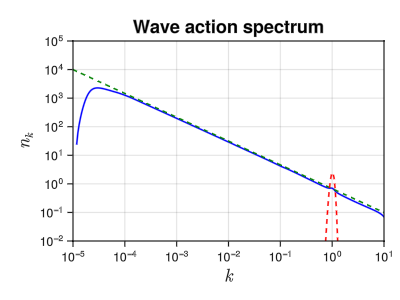
\includegraphics[width=0.4\textwidth]{images/MMT_inverse_256_[1.0e-5-10.0].png}
            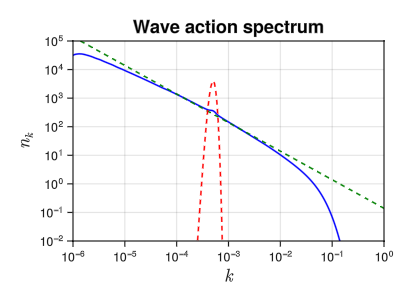
\includegraphics[width=0.4\textwidth]{images/MMT_direct_256[1.0e-6_1.0].png}
            \vspace{-0.5cm}
            \caption{Inverse and direct cascades from WavKinS.}
            \label{fig:cascdir}
    \end{figure}
    \begin{figure}[ht]
        \centering
        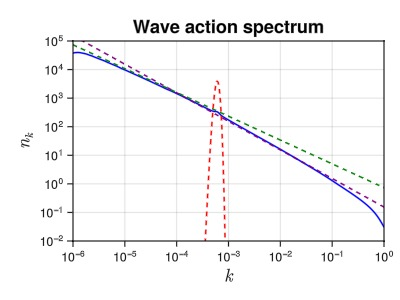
\includegraphics[width=0.5\textwidth]{images/double_cascade3.jpg}
        \vspace{-0.5cm}
        \caption{Double cascade from WavKinS.}
        \label{fig:cascdouble}
    \end{figure}
    In the direct cascade the inertial range is smaller, it is however the longest we could reproduce. In the range $10^{-6}$-$10^{-4}$ in figure \ref{fig:cascdir}  the forcing and dissipation terms are not negligible, we had however to distance the forcing term from the lower end of the grid to avoid divergences during time evolution. \\
    As a last example we simulated the situation where an inertial range is present on both sides of the forcing in $k$-space. The results, again in remarkable agreement with theoretical predictions, are in figure \ref{fig:cascdouble}. \\
    \subsection{Future work}

    The novel contribution of this thesis consisted in the analysis we presented of the higher order WKE for the MMT model. 
    Our work, however, can be at best called preliminary. There are many other approaches to try. One could include the frequency shift with a generic $\beta$, to see if it influences the presence of divergences. One could also include higher order diagrams in the derivation, to check if there is any cancellation. On the numerical side one could forcefully impose a cutoff on the diverging denominator, to at least see the qualitative deviation of possible stationary states from the KZ spectra.\\
    It is an open question whether nontrivial resonances still exists in higher dimensions, and for which dispersion relations they do.\\
    Another possible route would be to examine the higher order kinetic equation in three wave systems, and check whether such divergences appear as well. 

    
